\section{Production reconstructions, graded by measured reliability}
\label{sec:production}
We now return to the three production endpoints.  They are \emph{demonstrations} of the
measured instrument, not the contribution itself.  Every component below carries three
things: (i) its evidence grade, (ii) the probe that produced it, and (iii) that probe's
measured reliability on \benchname{} from Sec.~\ref{sec:howfar}.  One caveat applies to
everything in this section.  The reliabilities were measured on \benchname{} under its
own observability and serving regime.  Carrying those error rates over to a frontier
production deployment is an assumption about external validity, because the benchmark
and production are different populations: CPU serving against accelerated serving, and
known checkpoints against frontier stacks.  In symbols, $P_{\rm production}\neq P_{\rm
benchmark}$.

\begin{figure}[t]\centering
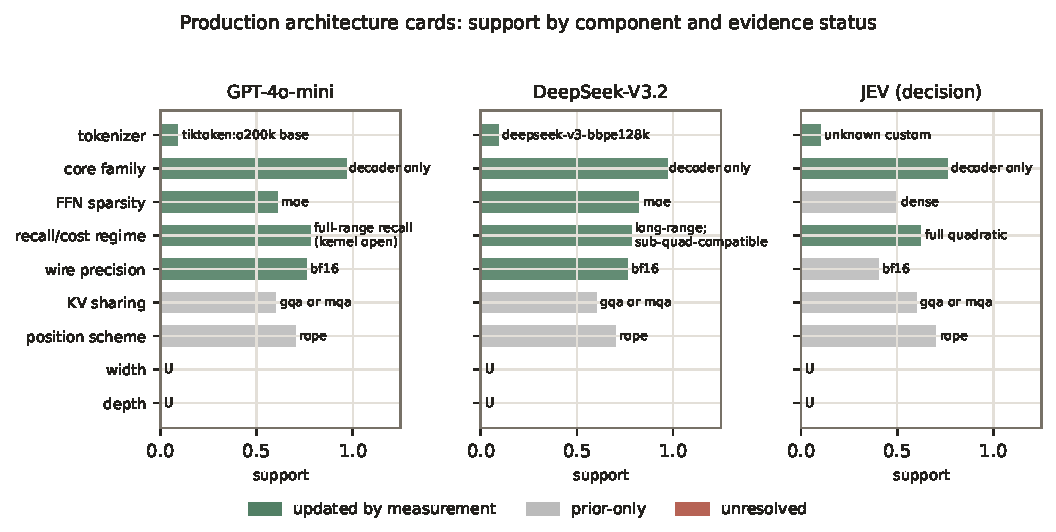
\includegraphics[width=\textwidth]{figures/fig_v4_cards.pdf}
\caption{Production architecture cards: per-component support with evidence status
(green = updated by measurement, grey = prior-only, red/U = unresolved).  Generated from
the recorded scan posteriors; the attention row carries the powered follow-up's reading,
not the recall-only prior.}
\label{fig:cards}
\end{figure}

\subsection{GPT-4o-mini: the worked reconstruction}
\label{sec:gptcase}
The eight-step progression (Fig.~\ref{fig:recongpt}) shows the instrument at work on an
opaque endpoint.  Each step says what it can establish and what it cannot.
\begin{enumerate}[nosep,leftmargin=1.6em,label=\textbf{\arabic*.}]
\item \textbf{Interface boundary.} An over-limit request reads the deployment contract
  straight from the error text: 16{,}384 maximum completion, 16{,}393-token accepted
  input (L1).  The model's documented capability is larger \cite{openaimini2024docs}.
  This is a fact about the interface layer, not the model (Sec.~\ref{sec:layers}).
\item \textbf{Tokenization.} Count differences on a fixed scaffold match
  \texttt{o200k\_base} and \texttt{o200k\_harmony} on all 18 strings.  That is a
  count-family identification with a proved tie (Prop.~\ref{prop:tok}), L2.
\item \textbf{Generation path.} A 24-token continuation whose latency rises with output
  length (23\,$\to$\,202\,ms) establishes the autoregressive-compatible generation
  contract, L2.  This is contract-level, not transformer-specific
  (Sec.~\ref{sec:familysplit}).
\item \textbf{Attention/state regime.} 18 of 18 needle retrievals succeed through 8{,}225
  tokens, which establishes full-range recall.  The attention kernel itself stays
  unseparated at these spans (L4; Fig.~\ref{fig:attncontrol}).
\item \textbf{KV sharing / positions.} GQA/MQA and RoPE appear only as priors.  They
  are shown in grey and never counted as recovered.  The discriminators that would decide
  them are recorded by name.
\item \textbf{Numeric regime.} The logprob lattice is consistent with bf16 (support 0.76),
  L4 at the wire layer.
\item \textbf{Feed-forward.} Dense or MoE is ambiguous (0.61 against 0.39).  It is reported
  at the detector's measured \MoeAcc{} reliability, with the interleaved control
  returning a null.
\item \textbf{Width/depth.} Width is unresolved by access (the top-5 wall,
  Prop.~\ref{prop:rank}).  Depth is unresolved by confound (compute and queueing are
  tangled).  Both are U with named next experiments.
\end{enumerate}

\begin{figure}[t]\centering
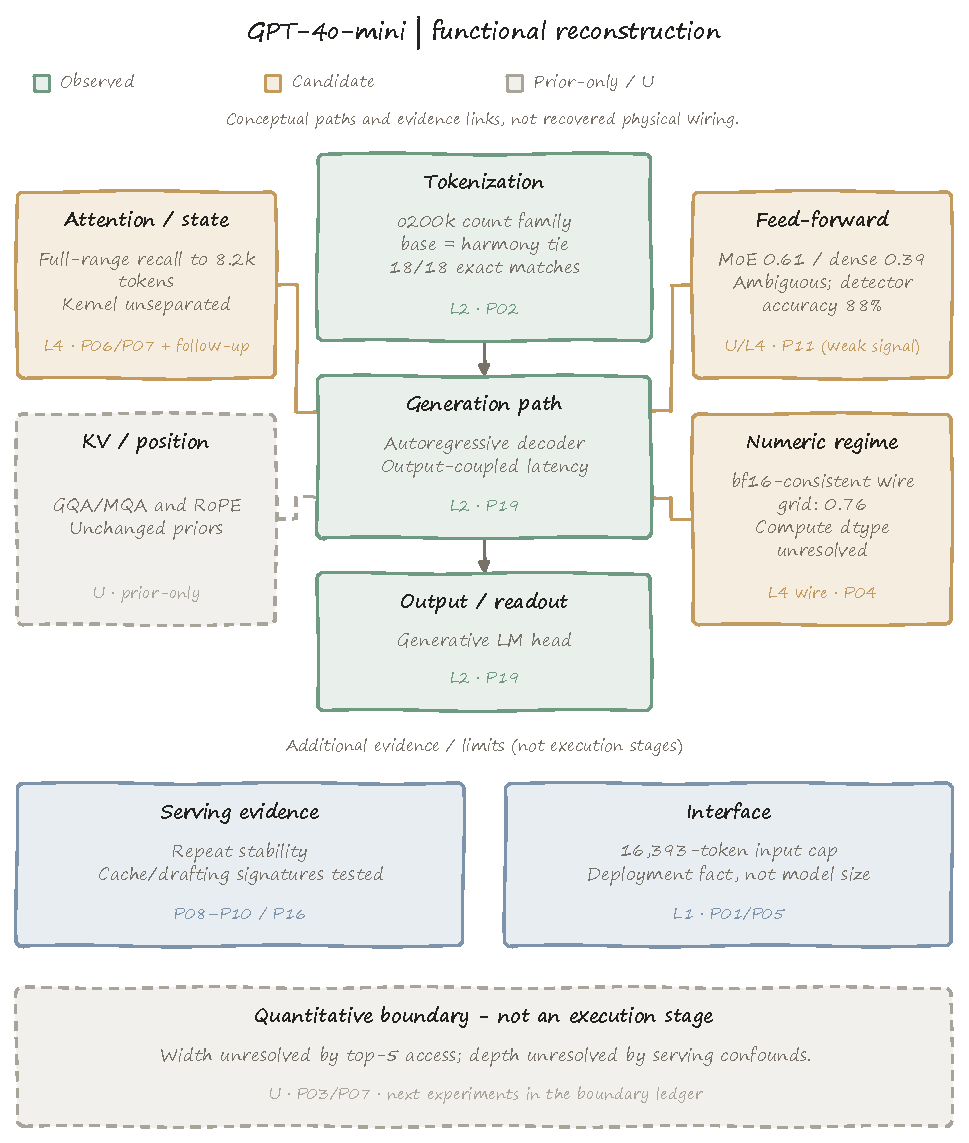
\includegraphics[width=\textwidth]{figures/fig_v4_recon_gpt.pdf}
\caption{GPT-4o-mini functional reconstruction.  Cards distinguish observed properties,
mechanism candidates, unchanged priors, and unresolved components.  Arrows show
conceptual functional order; side links associate evidence with a component, not
measured physical wiring.  The quantitative boundary is separate from the path.}
\label{fig:recongpt}
\end{figure}

\begin{table}[h]\centering\small
\caption{GPT-4o-mini: reconstructed components.  ``Bench'' is the detector's measured
accuracy on \benchname{}; grey rows are prior-only (no updating evidence).}
\label{tab:gptcard}
\begin{tabularx}{\textwidth}{@{}l Y c l Y@{}}
\toprule
\textbf{Component} & \textbf{Reconstruction} & \textbf{Grade} & \textbf{Bench} & \textbf{Basis}\\
\midrule
Input/output boundary & 16{,}393-token deployment cap; 16{,}384 max completion & L1 & - & error text; docs note larger model capability\\
Tokenizer & o200k count family (base$=$harmony tie) & L2 & 18/24 exact & 18/18 fixed-scaffold count matches (Prop.~\ref{prop:tok} tie)\\
Generation path & AR-compatible contract & L2 & 25/25 & 24-token continuation; latency scales with output\\
Transformer vs SSM & transformer-consistent, short span & U & 8/8 decided & engine decode TBT 11\,ms flat, CI $[-74,+86]$\,\textmu s/tok/1k (noise-dominated)\\
Attention regime & full-range recall to 8{,}225 tokens & L4 & - & 18/18 needle conditions; prefill exponent \GptFreshExp{} \GptFreshCI{} at $\le$15k\\
Wire numerics & bf16-consistent lattice & L4 & 80\% & P04 grid match\\
Feed-forward & dense/MoE ambiguous (MoE 0.61) & U & 88\% & domain timing weakest; interleaved control null\\
KV / position & GQA/MQA, RoPE (priors only) & U & - & no updating evidence; named next experiments\\
Width / depth & unresolved & U & - & top-5 access wall (Prop.~\ref{prop:rank}); compute$\times$queueing confound\\
\bottomrule
\end{tabularx}
\end{table}

\begin{figure}[t]\centering
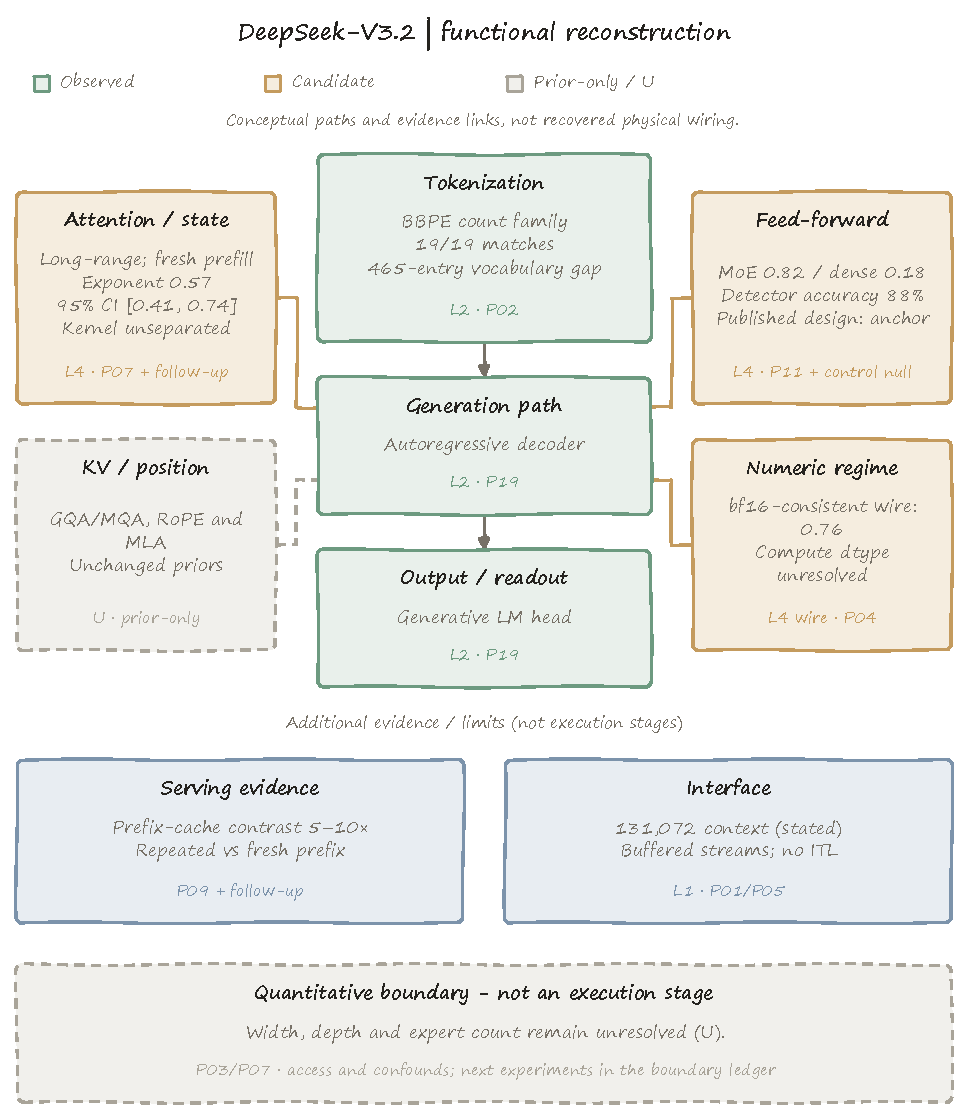
\includegraphics[width=\textwidth]{figures/fig_v4_recon_deepseek.pdf}
\caption{DeepSeek-V3.2 functional reconstruction: MoE-leaning feed-forward and
long-context evidence with unresolved alternatives.  Side links are evidence
associations, not physical wiring; the published design is an evaluation anchor,
not a measurement.  Width, depth, and expert count remain unresolved.}
\label{fig:recondeep}
\end{figure}

\subsection{DeepSeek-V3.2}
The same battery reconstructs a BBPE count-family tokenizer (19 of 19 matches), an
autoregressive decoder path, and a stated 131{,}072-token context.  Two claims carry
the paper's production weight.

\paragraph{MoE-leaning feed-forward.}  The domain and jitter signatures give MoE 0.82
against dense 0.18, and the published design is indeed MoE.  But our own benchmark says
this class of detector is only \MoeAcc{} accurate.  So we report the lean \emph{and} the
discount together.  The interleaved, length-matched, one-token control (10 randomised
blocks with domain-label permutation) does not reject the null of no domain effect on
either endpoint, which weakens the timing discriminator.  The jitter signature remains.
Grade: L4, mechanism-consistent with an independent published anchor.  Not L2.

\begin{figure}[t]\centering
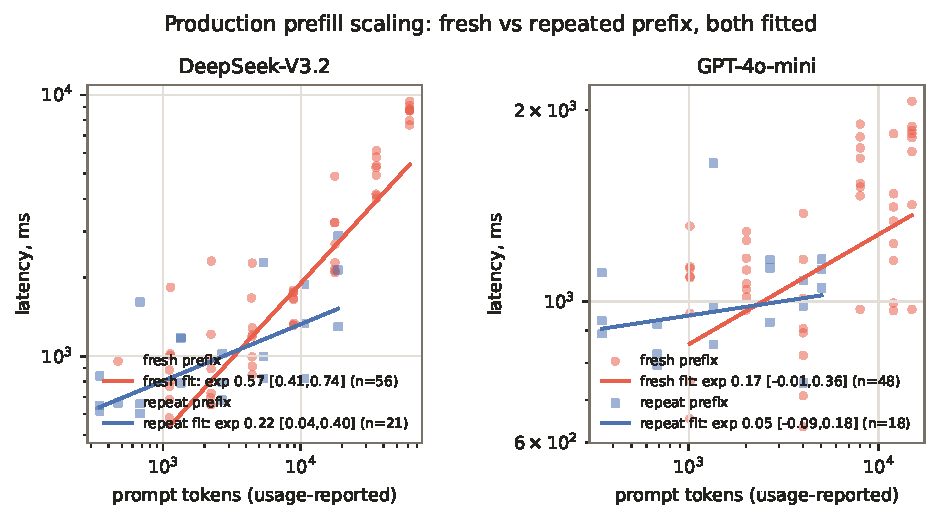
\includegraphics[width=\textwidth]{figures/fig_v4_prodscaling.pdf}
\caption{Production prefill scaling, powered follow-up: fresh-nonce (red) against
repeated-prefix (blue), both fitted with the same log-log model.  DeepSeek's fresh
exponent is sub-quadratic (\DsFreshExp{}, CI \DsFreshCI{}, $n$=\DsFreshN{});
GPT-4o-mini's prefill is overhead-dominated at these spans (\GptFreshExp{}, CI
\GptFreshCI{}, $n$=48).  Exponents constrain the attention node; they do not uniquely
select a kernel (Fig.~\ref{fig:attncontrol}).}
\label{fig:prodscaling}
\end{figure}

\paragraph{Fresh-prefix prefill scaling.}  The v2 comparison mixed a fitted
repeated-prefix curve with eight unfitted fresh-nonce points.  Most of what it showed
was a prefix-cache artifact.  The powered follow-up (Fig.~\ref{fig:prodscaling}) fits
both curves with the same log-log model on randomised trials.  A log-log fit means we
plot the logarithm of time against the logarithm of context length; the slope of that
line is the scaling exponent, where 1 means linear and 2 means quadratic.  The fresh
exponent is \DsFreshExp{} (95\% CI \DsFreshCI{}, $n=\DsFreshN$); the repeated-prefix
exponent is \DsRepeatExp{} (\DsRepeatCI{}, $n=\DsRepeatN$).  The fresh curve is
sub-quadratic, which is compatible with the documented sparse attention
\cite{deepseekai2025v32}.  But our same-hardware control (Fig.~\ref{fig:attncontrol})
shows that small dense models at short spans also look sub-quadratic.  So the exponent
does not \emph{select} DSA.  It narrows the attention node to candidates that are
compatible with sub-quadratic scaling.  Grade: L4, not L2.

\begin{figure}[t]\centering
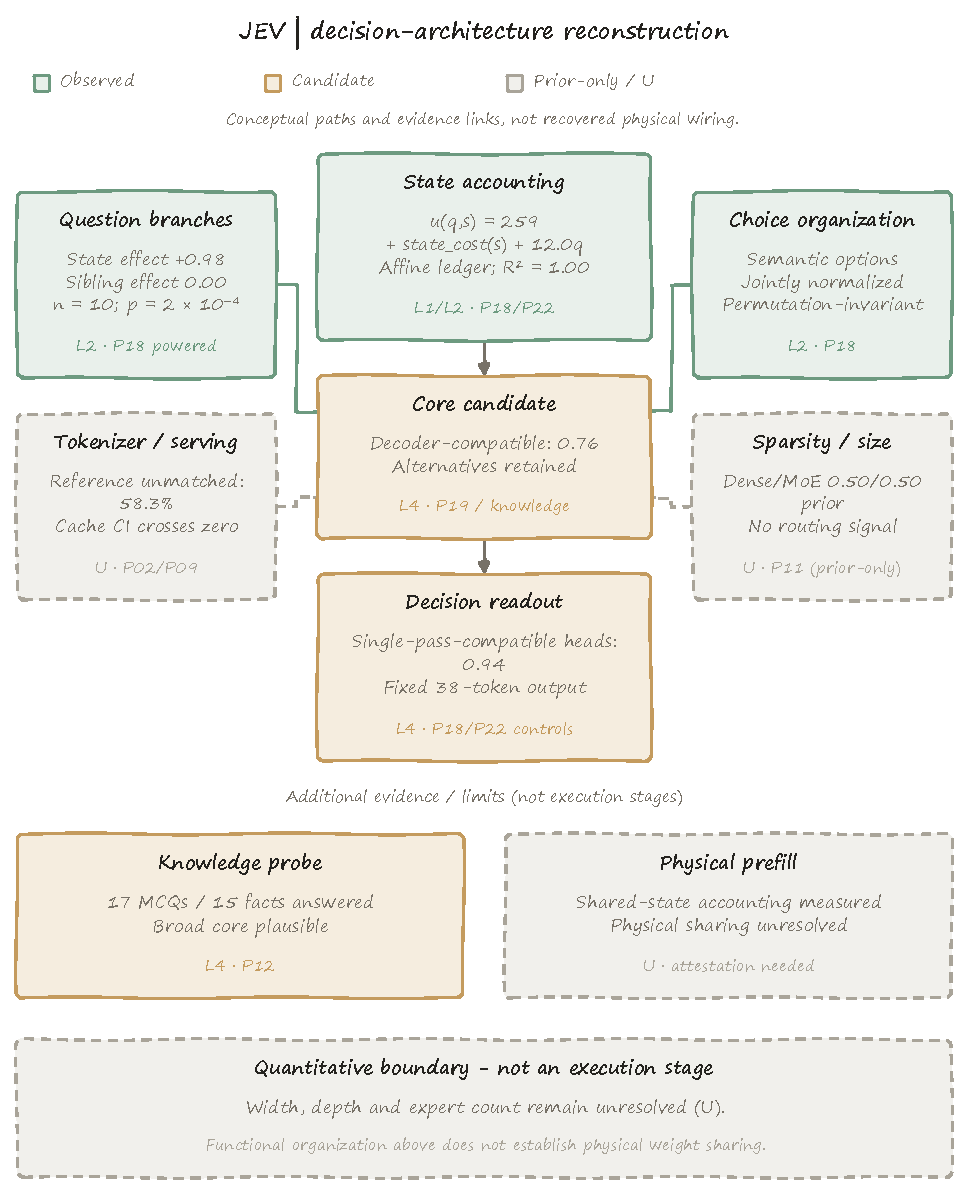
\includegraphics[width=\textwidth]{figures/fig_v4_recon_jev.pdf}
\caption{JEV's decision reconstruction: measured state accounting, isolated branches,
and normalized choices alongside a candidate core and single-pass-compatible readout.
Side links associate evidence; neither these links nor the affine ledger establish
physical weight sharing.  The quantitative boundary remains unresolved.}
\label{fig:reconjev}
\end{figure}

\subsection{JEV: a cross-contract generality test, powered}
JEV plays one specific role in this paper.  It is the \emph{cross-contract generality
test}: proof that the instrument is not a trick that only works on text-generation
APIs, but also works on a decision endpoint with a different interface contract.  Its
reconstruction is unchanged in kind and stronger in evidence.  The shared-state
accounting follows an exact linear ledger, $u(q,s)=259+\mathrm{state\_cost}(s)+12.0q$
with $R^2=1.00$: a fixed 259 tokens, plus the cost of the state, plus 12 tokens per
question.  The branches are isolated, the semantic choices are normalized, and the
readout is a fixed 38 tokens.  In v2 the branch-isolation claim rested on three trials.
The powered follow-up runs $n=\JevSecrets{}$ fresh secrets $\times$ \{baseline,
secret-in-state, secret-in-sibling\} in randomised order.  Planting the secret in the
shared state moves the answer by +\JevStateEff{}; planting it in a sibling question
moves it by \JevSibEff{}; the permutation test gives $p=\JevPermP$
(Fig.~\ref{fig:jevpower}).  Isolated branches over a shared state are now an L2-grade
measured property of this endpoint, not a three-trial hint.

\begin{figure}[t]\centering
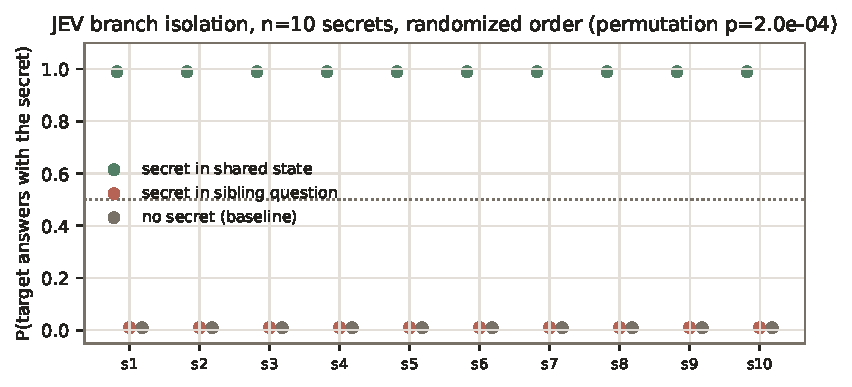
\includegraphics[width=.8\textwidth]{figures/fig_v4_jevpower.pdf}
\caption{JEV branch isolation, powered: $n$=10 fresh secrets, randomised order.  Secrets
in the shared state are used (+0.98); secrets in sibling questions are invisible (0/10,
permutation $p=2\times10^{-4}$).}
\label{fig:jevpower}
\end{figure}
